
\documentclass[10pt, a4paper]{article}

\usepackage[top=1in, bottom=1in, left=1in, right=1in]{geometry}
%\usepackage{setspace}
%\onehalfspacing
\usepackage{graphicx}
\usepackage{float}

\usepackage{subfig}
\usepackage{amsmath}

\usepackage{amssymb}
\usepackage{fancyhdr}
\usepackage{listings}
\usepackage{textcomp}
\usepackage{upquote}
\pagestyle{fancyplain}

\renewcommand{\arraystretch}{1.5}

\begin{document}
\lhead{Jay Mundrawala}
\rhead{ECE 481 - Homework 3}

\begin{enumerate}
    \setcounter{enumi}{2}
  \item A 1D signal $f(m) = (1,1,0,0)$ is observed through a noisy, linear system 
    $g(m) = h(m) * f(m) + n(m)$, where $h(m)=(1,2,1,0)$ and a particular 
    noise realization is $n(m)=(0.1,-0.1,0,0.1)$.
    \begin{enumerate}
      \item Plot $f(m), h(m), n(m)$, and $g(m)$.
        \begin{figure}[h!]
          \centering
          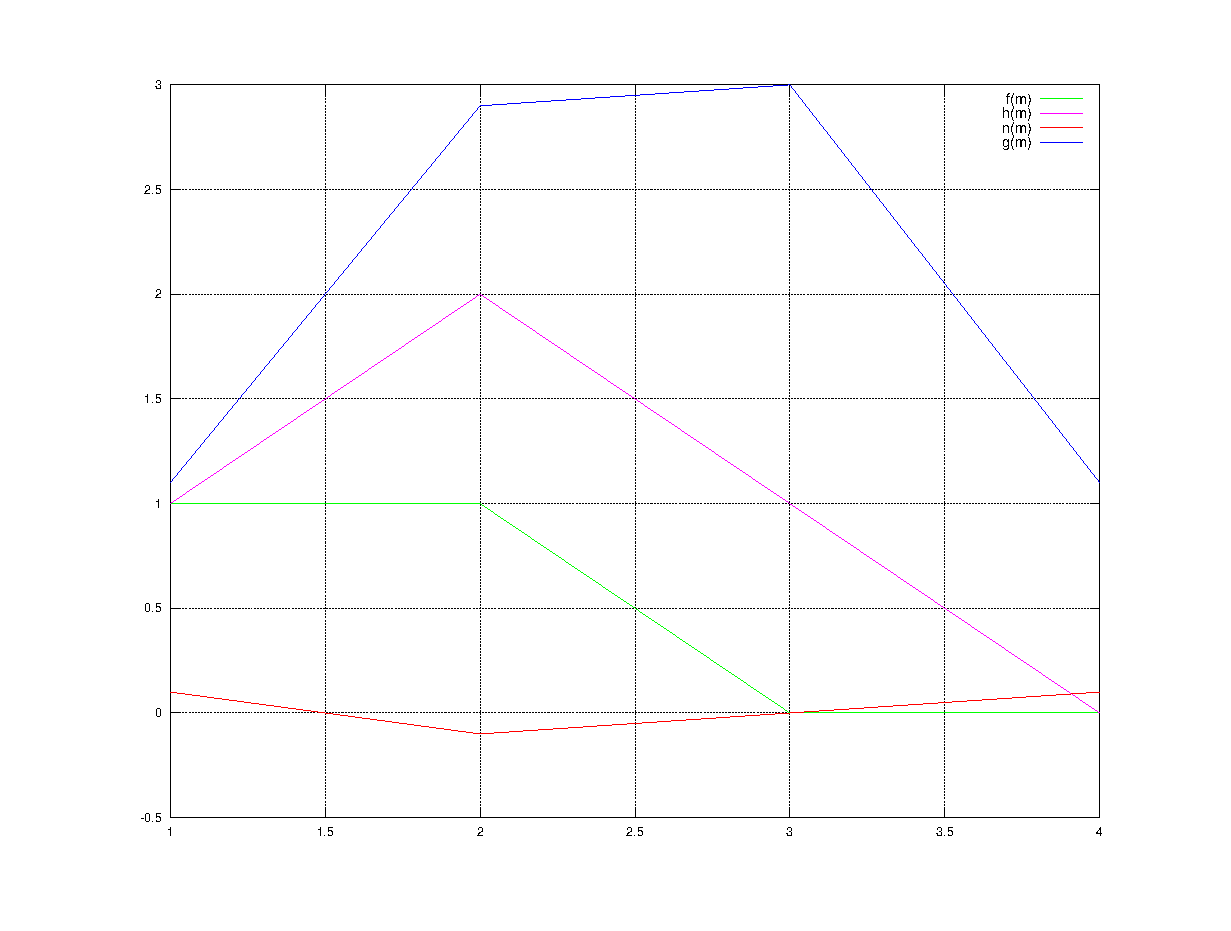
\includegraphics[scale=0.55]{../data/3a.eps}
          \caption{Plots for 3a}
        \end{figure}
      \item Calculate the DFTs $F(k), H(k), N(k)$, and $G(k)$. Plot their
        magnitudes $|F(k), |H(k)|, |N(k)|,$, and $|G(k)|$.
        \begin{figure}[h!]
          \centering
          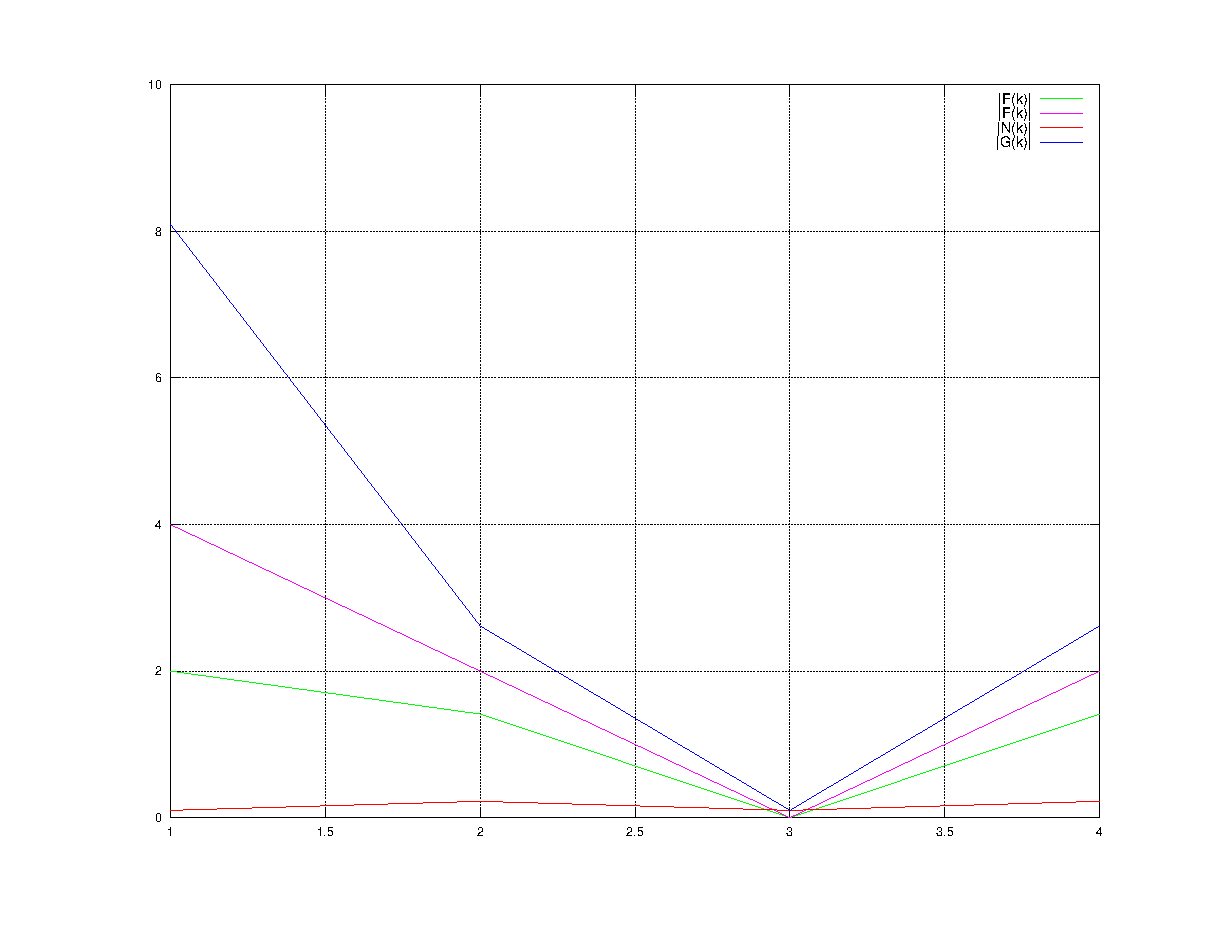
\includegraphics[scale=0.55]{../data/3b.eps}
          \caption{Plot for 3b}
        \end{figure}
      \item Can you apply the inverse filter to restore $f(m)$?

        No because there is a zero in H.
    \end{enumerate}
    \pagebreak
  \item Write a MATlAB program to do histogram equalization as described in class.

    The source is in \textit{../src/hist\_eq.m}. The results are shown in Figure \ref{fig:4}.
    \begin{figure}[h!]
          \centering
          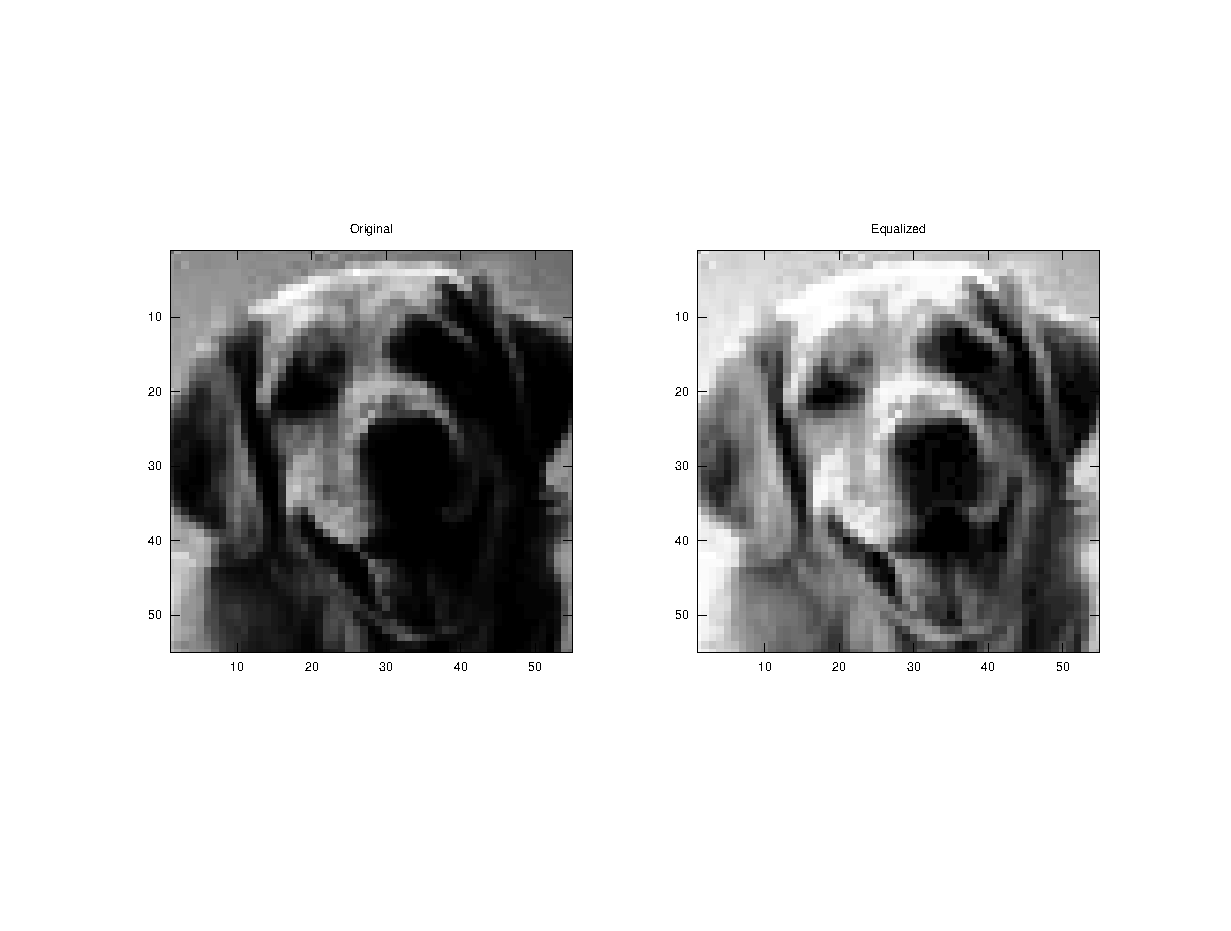
\includegraphics[]{../data/4.eps}
          \caption{Applying the histogram equalization method to dog1.tif}
          \label{fig:4}
    \end{figure}
  \item Write the following functions in MATLAB:
    \begin{description}
      \item[Function A] - Apply a $K$ x $K$ median filter to an $M$ x $N$ image.
        
        The source is in \textit{../src/median\_filter.m}. The results are shown in Figure \ref{fig:5a}
        \begin{figure}[h!]
          \centering
          
\includegraphics[]{../data/5a.eps}
          \caption{Applying the median filter to diver.tif}
          \label{fig:5a}
        \end{figure}       
      \item[Function B] - Perform direct linear convolution between an $M$ x $N$ image f and
        a $K$ x $K$ kernel h.

        The source is in \textit{../src/conv2\_linear.m}. The results are shown in Figure \ref{fig:5b}.
        \begin{figure}[h!]
          \centering
          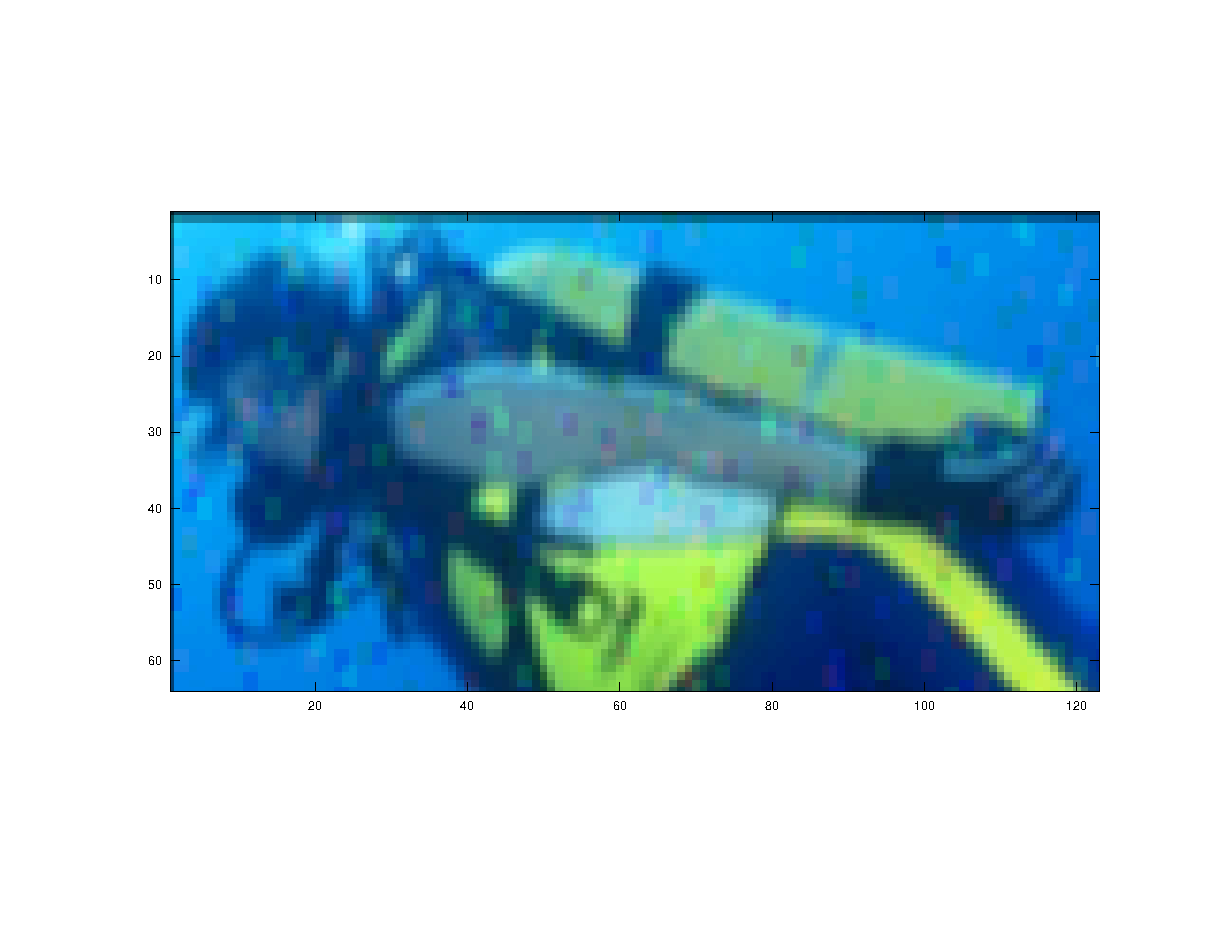
\includegraphics[width=170px]{../data/5b.eps}
          \caption{Applying a low pass filter to diver.tif}
          \label{fig:5b}
        \end{figure}       
    \end{description}
  \item Write a function that calls the linear convolution function using the Prewitt operators
    and computes an edge map of the monochrome image \textit{bacteria.tif} using $threshold=100$
    to make the binary edge mag $g_t(m,n)$ from the gradient magnitude image.

    The source is in \textit{../src/prewitt\_filter.m}. The results are shown in Figure \ref{fig:6}.
    \begin{figure}[h!]
      \centering
      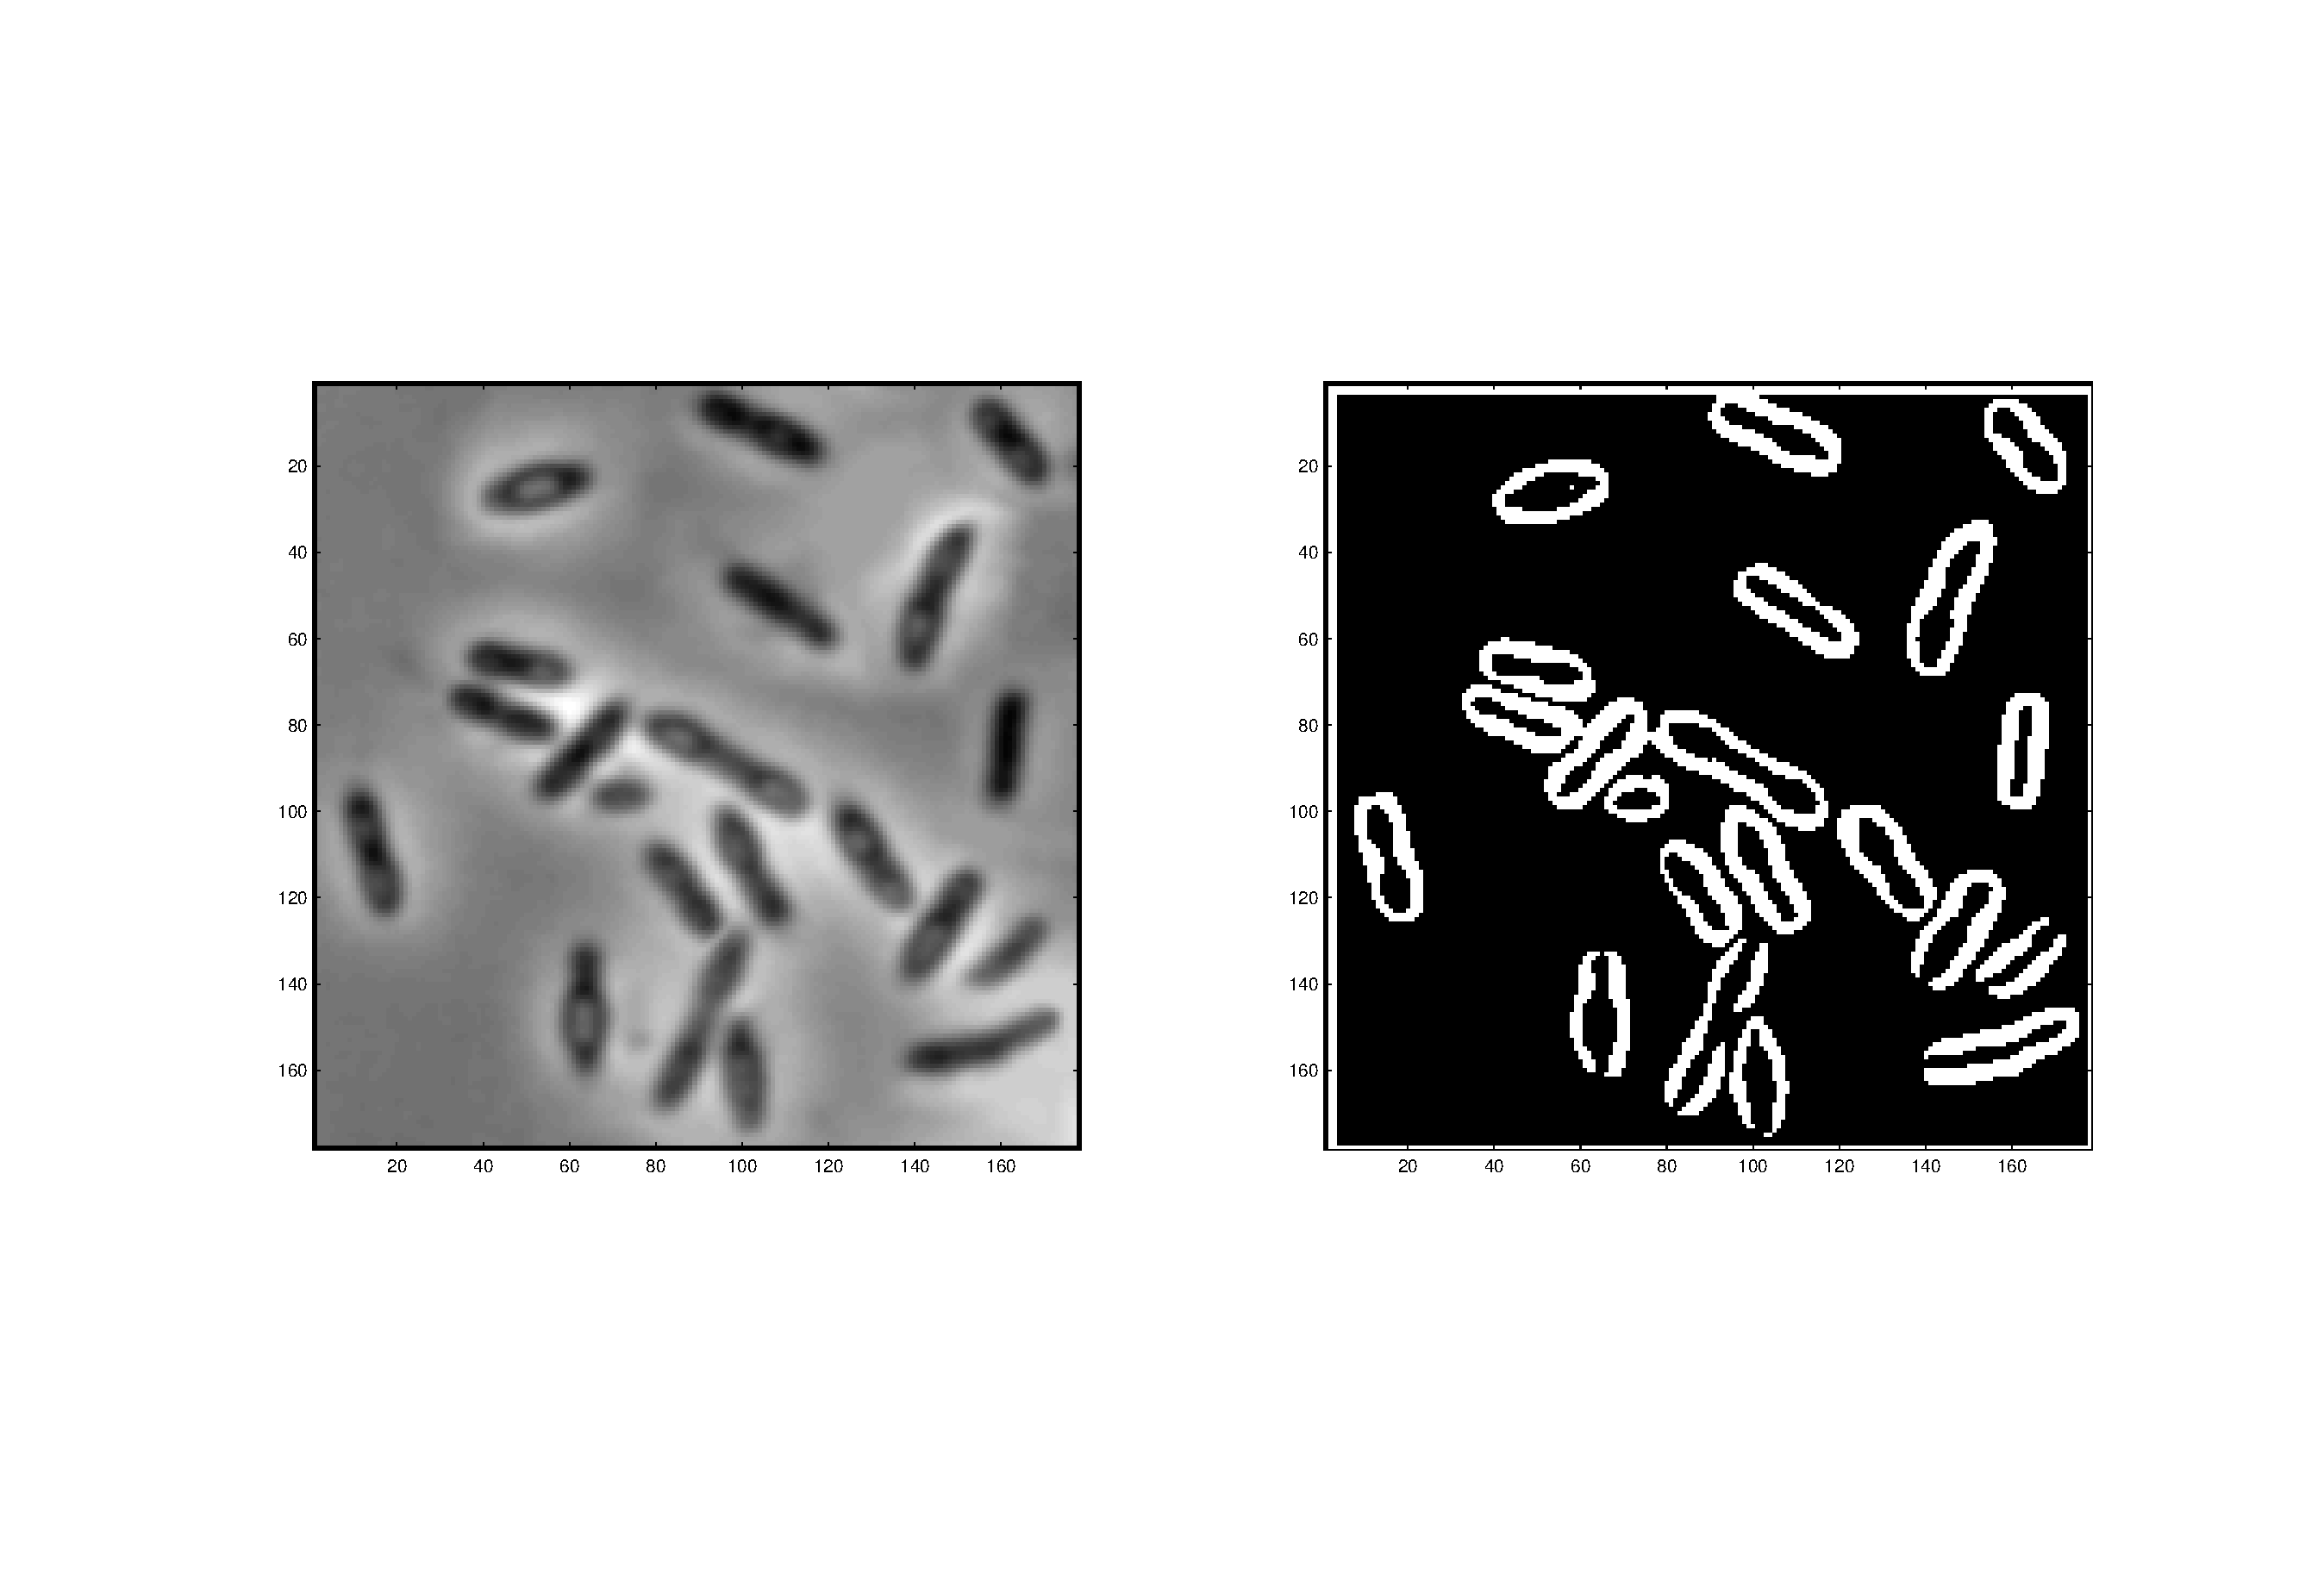
\includegraphics[width=0.95\textwidth]{../data/6.eps}
      \caption{Applying the Prewitt operators to bacteria.tif} 
      \label{fig:6}
    \end{figure}
\end{enumerate}

\end{document}

